\section{First Section}

\subsection{Block section}

\begin{frame}{Blocks}
	\begin{alertblock}{Alertblock}
		\begin{itemize}
			\item This is an alertblock
		\end{itemize}
	\end{alertblock}

	\pause

	\begin{block}{Normal Block}
		\begin{itemize}
			\item This is a normal block
			\item {\color{gray} There are more blocks!}
		\end{itemize}
	\end{block}

	\begin{exampleblock}{Example Block}
		\begin{itemize}
			\item This is an example block
		\end{itemize}
	\end{exampleblock}

	\begin{customblock}{Numbered (theorem-like) Custom Block}
		This is a theorem-like custom block
	\end{customblock}
\end{frame}





\subsection{Math section}

\begin{frame}{Math}
	\begin{theorem}[Theorem of me (2023)]
		This is a theorem using a custom color!
	\end{theorem}
	\begin{proof}
		This is a proof using a custom color!
	\end{proof}
\end{frame}





\subsection{Code section}

\begin{frame}[fragile]{Code}
Make the frame fragile!
\begin{lstlisting}[language=Java]
public boolean equals(Object other) {
    if (other == null) {
        return false;
    }
    if (!(other instanceof Product)) {
        return false;
    }
    Product product2 = (Product) other;
    if (getName().equals(product2.getName())) {
        if (getPrice() == product2.getPrice()) {
            return true;
        }
    }
    return false;
}
\end{lstlisting}

\end{frame}



\begin{frame}[fragile]{Code}
 \begin{lstlisting}[language=Java]
|{\colorbox{red!20}{public}| boolean equals(Object other) {
    |{\colorbox{red!20}{if}| (other == null) {
        |{\colorbox{green!20}{return}| false;
    |{\colorbox{green!20}{\}}|
    |{\colorbox{orange!20}{if}| (!(other instanceof Product)) {
        |{\colorbox{blue!20}{return}| false;
    |{\colorbox{blue!20}{\}}|
    |{\colorbox{red!20}{Product}| product2 = (Product) other;
    |{\colorbox{red!20}{if}| (getName().equals(product2.getName())) {
        |{\colorbox{green!20}{if}| (getPrice() == product2.getPrice()) {
            |{\colorbox{orange!20}{return}| true;
        |{\colorbox{orange!20}{\}}|
    |{\colorbox{blue!20}{\}}|
    |{\colorbox{red!20}{return}| false;
|{\colorbox{green!20}{\}}|
\end{lstlisting}

\end{frame}





\subsection{Image, Columns, Drawing section}
\begin{frame}{White Box Test vs. Black Box Test}
	\begin{columns}
		\begin{column}{0.55\textwidth}
			\textbf{Black Box Test}\\
			\begin{itemize}
				\item Implementierung unbekannt
				\item Anhand der Spezifikation entwickelt
				\item \texttt{Output == Expected Output}
			\end{itemize}
			\addSlideNo{9}{63-77}
			\addSheetEx{A}{10}{3}
			\vspace{0.1cm}

			\pause

			\textbf{White Box Test}\\
			\begin{itemize}
				\item Code bekannt
				\item Zeilenüberdeckung ...
			\end{itemize}
			\addSlideNo{11}{8-27}
		\end{column}
		\begin{column}{0.55\textwidth}

			\pause

			\begin{center}
				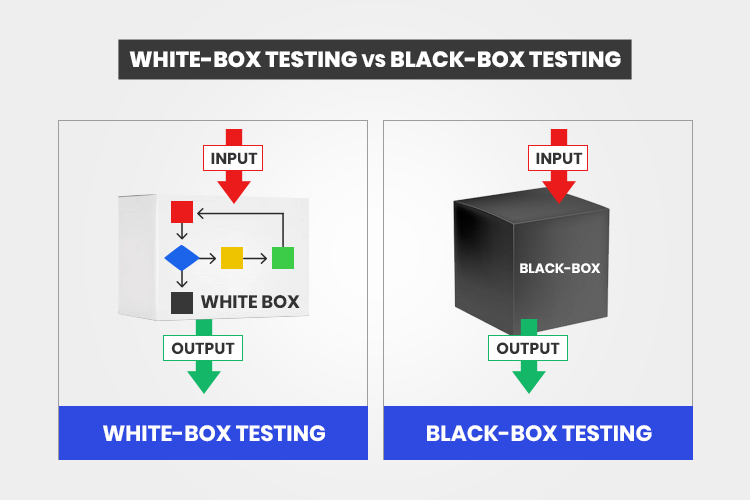
\includegraphics[width=\textwidth]{ressources/imgs/sample.jpg}
				{\tiny \url{https://www.temok.com/blog/wp-content/uploads/2020/10/Virus5.jpg}, Stand: 16.02.23}
			\end{center}

		\end{column}
	\end{columns}
\end{frame}



\begin{frame}{Drawing TikZ}
	\resizebox{\textwidth}{!}{
    	\begin{tikzpicture}[node distance=2cm]

% Nodes
\node (start) [block] {Start};
\node (n1) [block, below of=start] {Node 1};
\node (n2) [block, right of=n1, xshift=2cm] {Node 2};
\node (n3) [block, right of=n2, xshift=2cm] {Node 3};
\node (n4) [block, right of=n3, xshift=4cm] {Node Extra};

% Lines
\draw [line] (start.north) to [bend left=90, xshift=1cm, yshift=1cm] (n1.east);
\draw [line] (n1.south) to [bend right=45] node [pos=0.5, below] {yes} (n2.south);
\draw [line] (n2.north) -| node[anchor=west, yshift=0.5cm] {if True} ([yshift=3cm]n2.north) -| ([xshift=-4cm, yshift=3cm]n2.north) -| ([xshift=-1cm]start.west) -- (start.west);
\end{tikzpicture}

	}
	\addSheetEx{Ü}{8}{3}
\end{frame}
